\documentclass{beamer}
\usetheme{Frankfurt}
\usecolortheme{beaver}
\usepackage[utf8]{inputenc}
\usepackage{caption}
\usepackage{movie15}
\usepackage{tikz}
\usetikzlibrary{positioning, shapes.arrows}

\beamertemplatenavigationsymbolsempty
\setbeamertemplate{footline}[page number]
\AtBeginSection[]{
  \begin{frame}
  \vfill
  \centering
  \begin{beamercolorbox}[sep=8pt,center,shadow=true,rounded=true]{title}
    \usebeamerfont{title}\insertsectionhead\par%
  \end{beamercolorbox}
  \vfill
  \end{frame}
}

\title[Adversarial Attacks in autonomous driving]{Attacchi verso sistemi di apprendimento in ambito autonomous driving}
\subtitle{studio e implementazione in ambiente simulato}
\author{Niccolò Piazzesi}
\institute[Unifi]{
    Università degli Studi di Firenze \\

    Scuola di Scienze Matematiche, Fisiche e Naturali \\

    Tesi Di Laurea in Informatica \\

    Relatore:  Dott. Andrea Ceccarelli \\

    Anno Accademico 2019-20
}

\date{10 Luglio 2020}


\begin{document}

\begin{frame}[plain]
    \titlepage
\end{frame}


\section{Introduzione}
\begin{frame}
    \begin{columns}
        \begin{column}{0.6\textwidth}
            \begin{figure}
            \includegraphics[width=\textwidth]{auto}
            \end{figure}
        \end{column}
        \begin{column}{0.4\textwidth}
            I veicoli a guida autonoma usano le reti neurali per  processare le immagini raccolte da una videocamera e scegliere l'azione da compiere.
        \end{column}
    \end{columns}
\end{frame}
\begin{frame}
    \begin{columns}
        \begin{column}{0.5\textwidth}
            \includegraphics[width=\textwidth]{adv}
        \end{column}
    \begin{column}{0.5\textwidth}
       \begin{block}{ Adversarial Attack}
        modifica impercettibile all'input di una rete neurale, in grado
        di causare un errore di classificazione.
       \end{block}
    \end{column}
    \end{columns}
\end{frame}

\begin{frame}
    \begin{block}{Lavoro svolto}
        Iniezione di  adversarial attacks all'interno di un veicolo a guida autonoma in ambiente simulato.
    \end{block}
   \begin{block}{Motivazione}
       Se un attaccante riuscisse ad avere accesso alle immagini della videocamera prima che vengano processate, potrebbe
       modificarle e causare un grave fallimento della macchina. Stabilire gli effetti di questi attacchi è fondamentale nella valutazione
       di robustezza dei veicoli a guida autonoma.
   \end{block}
\end{frame}

\section{Strumenti utilizzati}
\begin{frame}
    \frametitle{Carla}
    \begin{columns}
        \begin{column}{0.5\textwidth}
            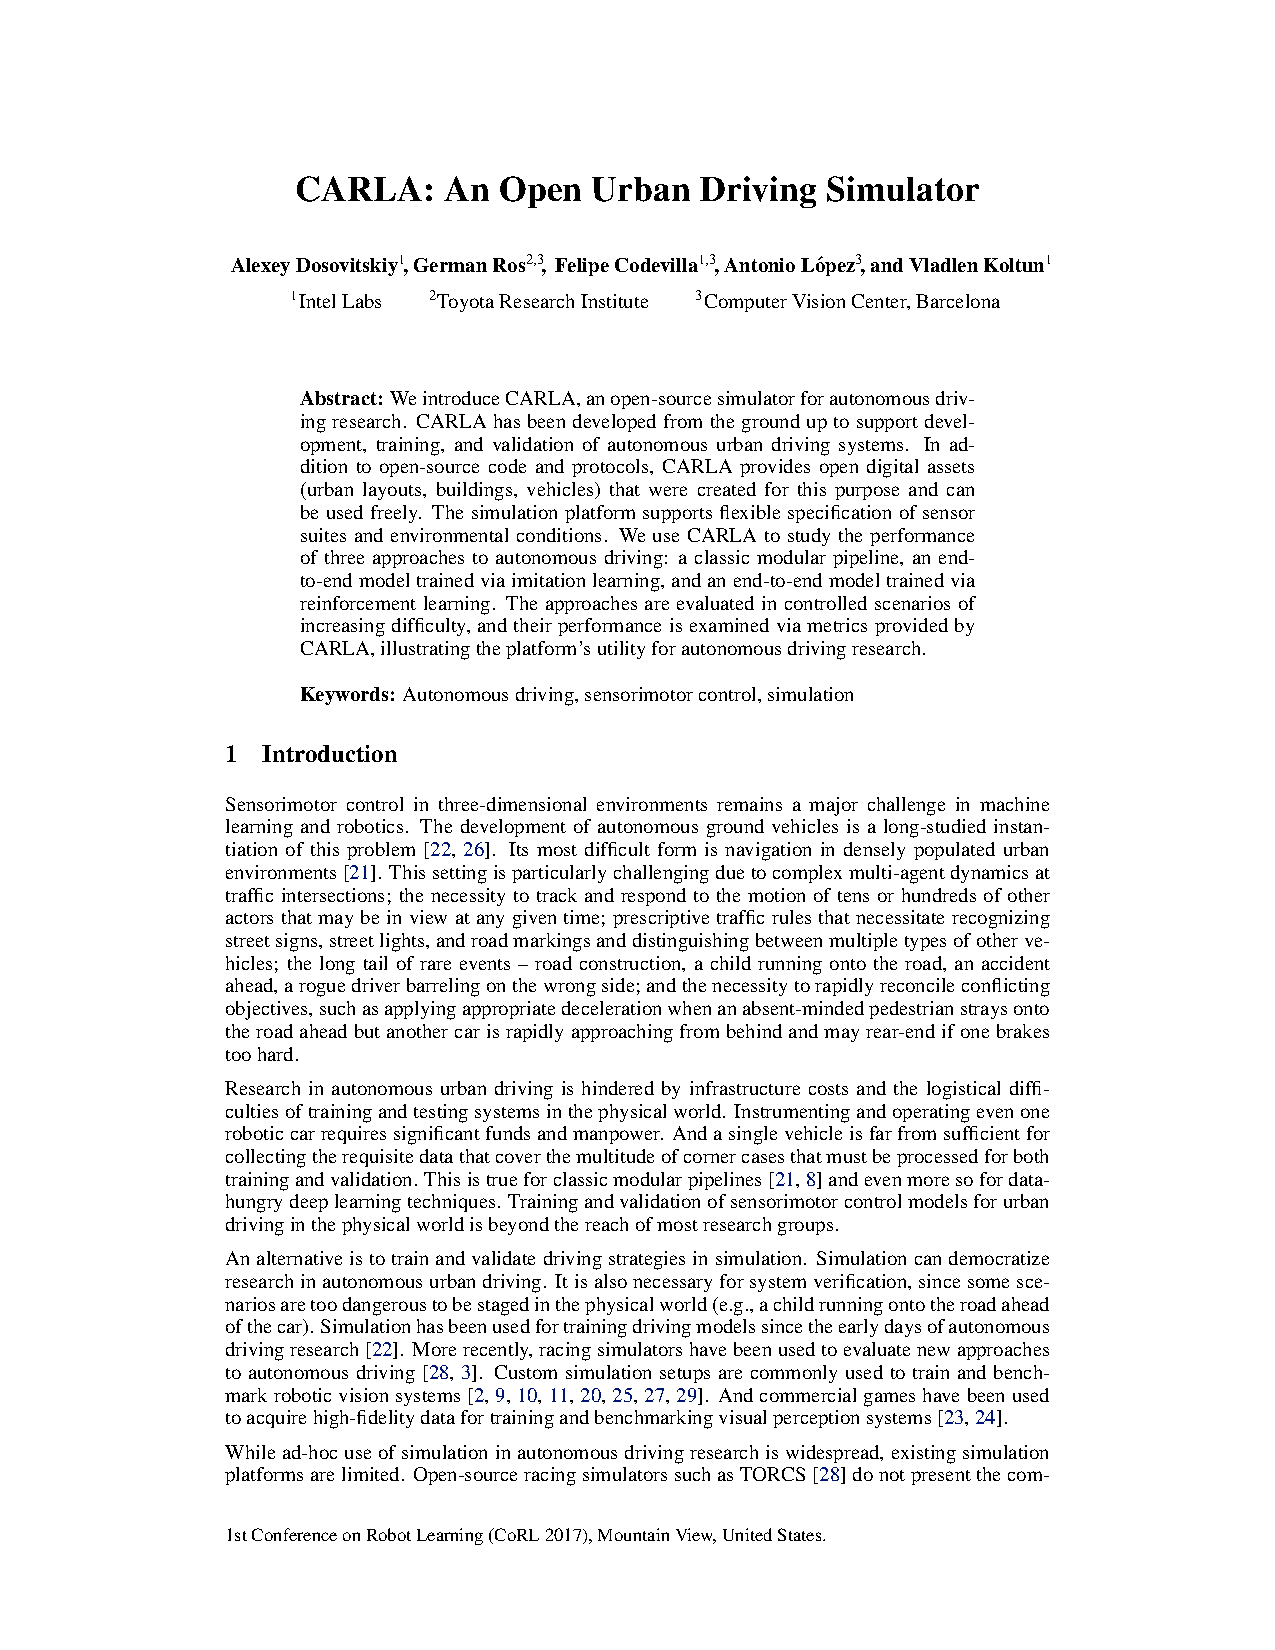
\includegraphics[width=\textwidth, height=0.3\textheight]{carla.jpg} 
            \includegraphics[width=\textwidth, height=0.3\textheight]{carlalogo.jpg} 
        \end{column}

        \begin{column}{0.5\textwidth}
              
    \begin{block}{Che cosa fornisce}
        Una simulazione realistica in 3D di un ambiente di guida urbana, con veicoli e pedoni.
    \end{block}
    
    \begin{block}{Come si usa}
        Architettura client-server. Il server controlla la simulazione e invia i dati raccolti da dei sensori ai client collegati.
        Un client controlla un veicolo e richiede informazioni attraverso la python API messa a disposizione.
    \end{block}
        \end{column}
    \end{columns}
\end{frame}


\begin{frame}
    \frametitle{LearningByCheating}
    
    \includegraphics[width=\textwidth]{agenti.png}

    Agente utilizzato durante la sperimentazione.

    L'immagine ottenuta da una  camera frontale viene processata insieme a velocità e comando di un agente supervisore da una rete neurale convoluzionale.
    
    L'output della rete è un insieme di 6 punti che rappresentano la posizione desiderata negli istanti successivi (waypoints).
    
    In base agli waypoints i controllori sterzano, accelerano o frenano.
\end{frame}

\begin{frame}
    \frametitle{Adversarial Robustness Toolbox (ART)}
    
    \begin{block}{\vspace*{-3ex}}
    Libreria python sviluppata da IBM per la ricerca sulla difesa dei modelli di Machine Learning dagli adversarial attacks.
    Mette a disposizione l'implementazione di attacchi, difese, e metriche di misura per la valutazione della robustezza di un modello, oltre a fornire
    un'interfaccia per usarla assieme a librerie esterne di Machine Learning (PyTorch, Tensorflow ecc\dots).
    \end{block}

    \begin{block}{\vspace*{-3ex}}
    L'implementazione degli attacchi si trova nel sottomodulo art.attacks. Sono divisi in 3 diverse categorie:
    Evasion Attacks, Poisoning Attacks, Extraction Attacks. Gli attacchi iniettati sono tutti Evasion Attacks.
    \end{block}
\end{frame}


    
\section{Iniezione, prove e risultati}
\begin{frame}
    \frametitle{Attacchi scelti}

            \begin{itemize}
               
                \item    Spatial Transformation (STA)
                    \includegraphics[width=0.8\textwidth]{spat.png}
                \item HopSkipJump (HSJ)
                    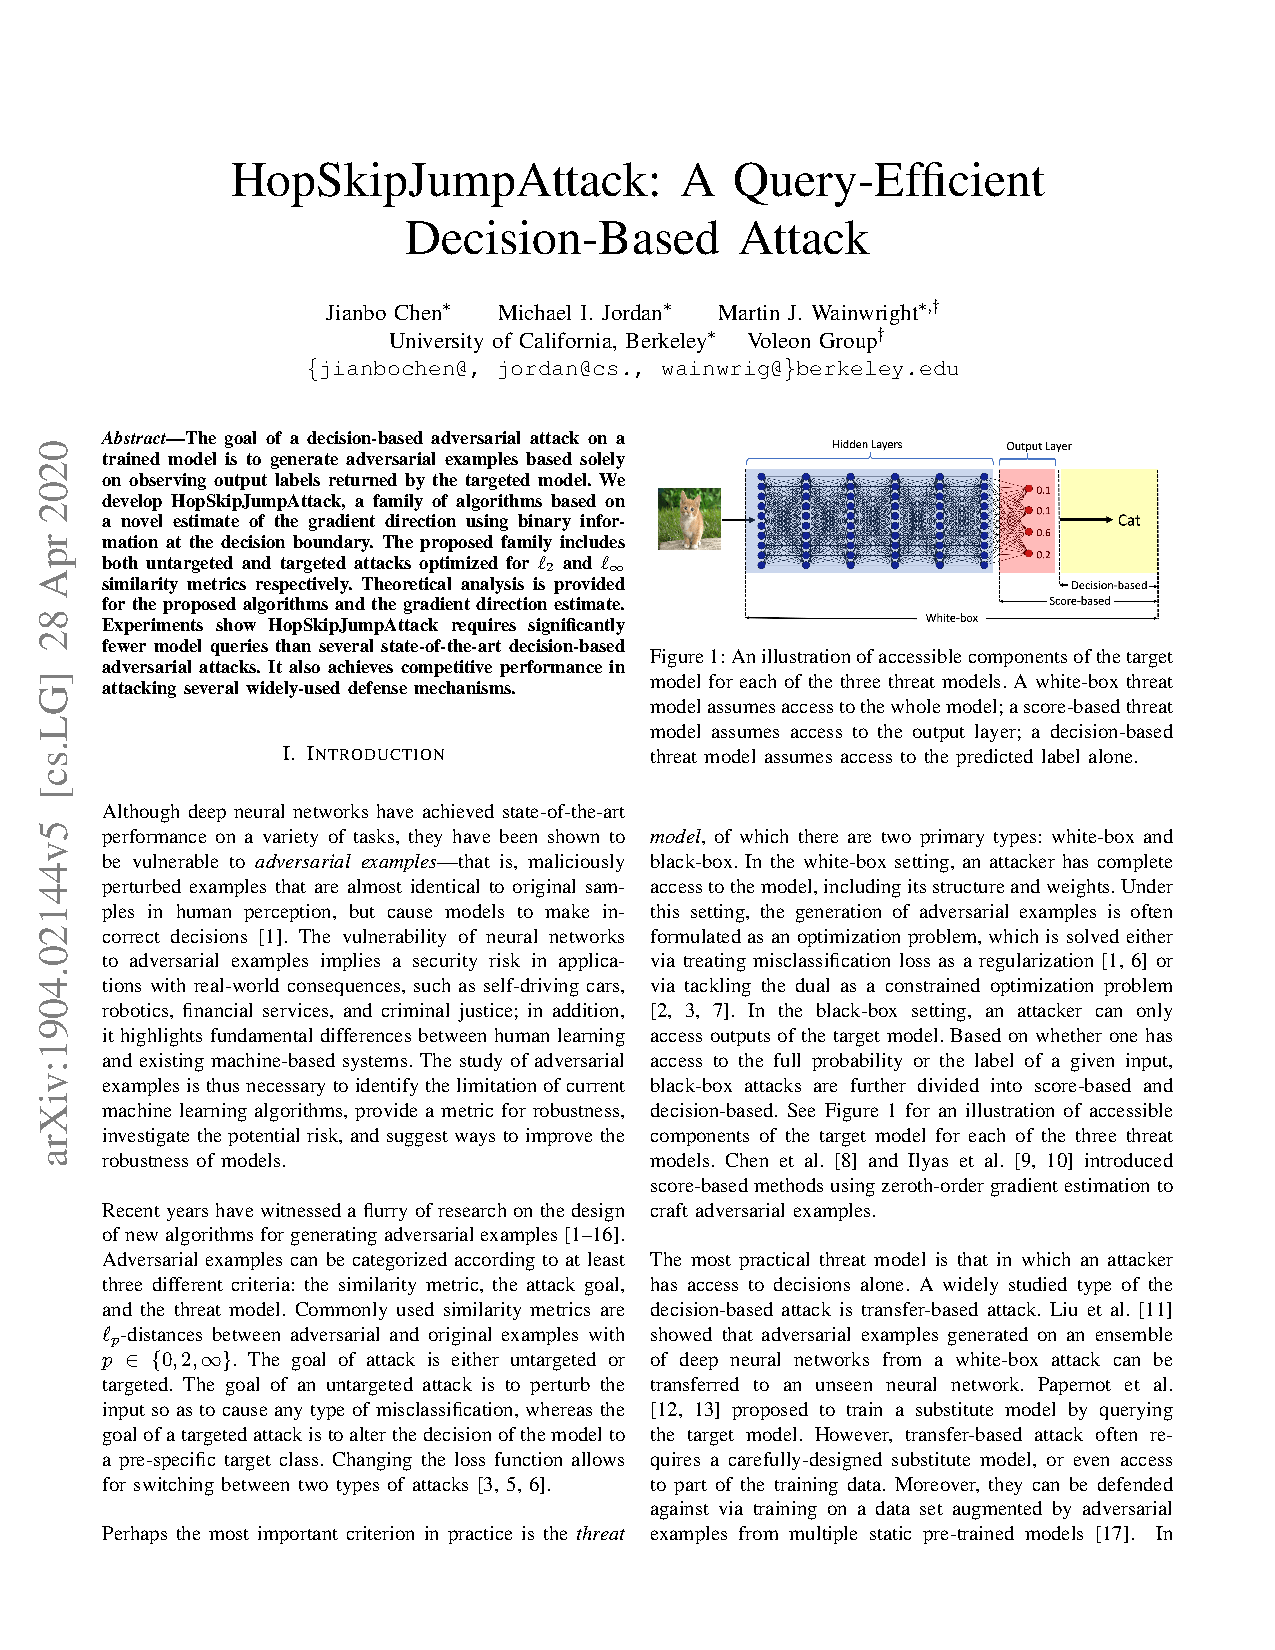
\includegraphics[width=0.8\textwidth]{hop.png}
                
            \end{itemize}
        
        

\end{frame}


\begin{frame}
    \frametitle{Attacchi scelti}
    \begin{itemize}
        \item Basic Iterative Method (BIM)
        \[X^{adv}_{0} = X, X^{adv}_{N+1} = Clip_{X,\epsilon}\{ X^{adv}_{N} + \alpha sign(\nabla _{X}J(X^{adv}_{N},y_{true})) \}\]
        \item NewtonFool (NF)
        
        Se $ F^l_s(x)$ rappresenta la probabilità della classe scelta dalla rete, trova una perturbazione d per cui $F^l_s(x + d) \approx 0$.
    \end{itemize}
\end{frame}

\begin{frame}
    \frametitle{Attacchi scelti}
    \begin{columns}
        \begin{column}{0.6\textwidth}
            \begin{itemize}
                \item Adversarial Patch\\
                \includegraphics[width =0.9\textwidth]{adversarial_patch.png}
            \end{itemize}  
        \end{column}
    \begin{column}{0.4\textwidth}
        \begin{block}{N.B}
            L'iniezione di questo attacco avrebbe richiesto la modifica dei modelli della simulazione per applicarci la patch. 
            A causa di alcune difficoltà nell'utilizzo dell'editor Unreal Engine, Adversarial Patch NON è stato iniettato.
        \end{block}  
    \end{column}
\end{columns}
\end{frame} 
\begin{frame}
    \frametitle{Iniezione degli attacchi}
    \begin{columns}
        \begin{column}{0.5\textwidth}
            \begin{tikzpicture}[
                roundnode/.style={circle, draw=green!60, fill=green!5, very thick, minimum size=7mm},
                squarednode/.style={rectangle, draw=red!60, fill=red!5, very thick, minimum size=5mm},
                ]
                %Nodes
                \node[squarednode]      (maintopic)                              {Attacco};
                \node[roundnode]        (uppercircle)       [above=of maintopic] {RGB};
                \node[roundnode]      (rightsquare)       [below=of maintopic] {RGB*};
                \node[squarednode]        (lowercircle)       [below=of rightsquare] {CNN};
                \node[roundnode]        (V)          [left=of lowercircle] {\scriptsize Velocità};
                \node[roundnode]        (C)          [right=of lowercircle] {\scriptsize Comando};
                
                
                %Lines
                \draw[->] (uppercircle.south) -- (maintopic.north);
                \draw[->] (maintopic.south) -- (rightsquare.north);
                \draw[->] (rightsquare.south) -- (lowercircle.north);
                \draw[->] (V.east) -- (lowercircle.west);
                \draw[->] (C.west) -- (lowercircle.east); 
                \end{tikzpicture}
            \end{column}
    \begin{column}{0.5\textwidth}
        \begin{block}{\vspace*{-3ex}}
            Modifica del codice di LBC. L'immagine raccolta ad ogni istante dalla camera frontale viene passata
            al metodo $generate$ fornito dall'ART, il quale  applica le modifiche (diverse per ciascun attacco). 
            La nuova immagine è quella effettivamente processata dalla rete.
            
        \end{block}
    \end{column}
    \end{columns}
\end{frame}

\begin{frame}
    \frametitle{Prove eseguite}
    \begin{block}{\vspace*{-3ex}}
        4 percorsi ripetuti tre volte con condizioni ambientali diverse. Ciascun percorso viene videoregistrato.
    \end{block}
   
    \begin{block}{\vspace*{-3ex}}
        In ogni percorso l'agente deve arrivare a una destinazione entro un tempo limite.
    \end{block}
        
    \begin{block}{\vspace*{-3ex}}
        La run fallisce se scade il tempo o avviene una collisione.
    \end{block}
    \begin{block}{\vspace*{-3ex}}
        Le prove sono state svolte prima senza nessun attacco iniettato (golden run) e successivamente iniettando uno a uno gli attacchi scelti.
        L'efficacia degli attacchi è stata valutata analizzando i video prodotti.
    \end{block}
    
\end{frame}


\begin{frame}
    \frametitle{Risultati}
    \begin{table}[h]
        \centering
        \begin{tabular}{|p{1.5cm}|p{1.5cm}|p{2cm}|p{1.5cm}|c|c|}
            \hline
            Attacco        &   Run terminate    &   stabilità traiettoria    &  semafori ignorati        & collisioni & timeout\\
            \hline
            Nessuno        &  12/12               &   ottima        &  0                       & 0          & 0 \\
            HSJ            &  6/12                &   bassa         &  9                        & 6          & 0 \\
            STA            &  7/12                &   discreta      &  0                        & 4          & 1 \\
            BIM            &  0/12                &   nulla         &  N/D                      & 12         & 0\\
            NF             &  3/12                &   bassa         &   13                      & 9          & 0 \\
            \hline
        \end{tabular}
        \caption{Riassunto dei risultati.}
        \label{tab:ria}
    \end{table}
\end{frame}
\section{Un esempio: iniezione di HopSkipJump}
\begin{frame}
    
    Golden Run:
        \includemovie[poster, controls, autoplay, autostop, mouse=true]{\textwidth}{0.3\textheight}{golden.avi}
    HopSkip Run:
        \includemovie[poster, controls, autoplay, autostop, mouse=true]{\textwidth}{0.3\textheight}{hop.avi}
\end{frame}
\section{Conclusioni}
\begin{frame}
    \begin{block}{\vspace*{-3ex}}
            Abbiamo iniettato alcuni degli attacchi forniti dalla libreria Adversarial Robustness Toolbox nel modello
            LearningByCheating.
    \end{block}

    \begin{block}{\vspace*{-3ex}}
        I dati raccolti hanno mostrato un sensibile calo dell'affidabilità della guida in presenza di tali attacchi.
\end{block}

\begin{block}{\vspace*{-3ex}}
    L'ART mette a disposizione anche varie difese contro gli adversarial attacks. La valutazione di queste difese potrebbe essere un interessante
    ampliamento di questo lavoro.

\end{block}
\end{frame}
\end{document}